\documentclass[11pt]{article}
\usepackage[margin=1in]{geometry}
\usepackage{amsmath, amssymb}
\usepackage{graphicx}
\usepackage{booktabs}
\usepackage{parskip}
\usepackage{hyperref}

\title{Exp B: sliding $\hat\beta_t$ on alternating-genre text}
\author{}
\date{\today}

\begin{document}
\maketitle

\section{Question}

The project proposal's stretch goal was: do per-context sliding $\hat\beta_t$
estimates beat batch fitting on heterogeneous text?  After Exp A, the
calibration framing of this question is moot --- the filter is not a
Guo-style temperature scaler (cf.\ Exp A findings).  The remaining
testable question: \emph{does the sliding $\hat\beta_t$ signal track corpus
genre transitions at all}?

\section{Setup}

Construct one mixed sequence by interleaving 4 WikiText-103 articles and 4
WritingPrompts stories, each truncated to 256 tokens: [wiki, WP, wiki, WP,
wiki, WP, wiki, WP] $\to$ 2048 tokens total.  Run the streaming Laplace
filter with $\sigma_0 = 0.5$ and memory\_decay $\gamma \in \{0.90, 0.95,
0.98, 0.99, 1.00\}$.  Within each chunk, exclude a 20-token boundary
window on each side before averaging (per the seam-confound caveat raised
in the Exp A audit).

\section{Result}

\begin{figure}[h]
\centering
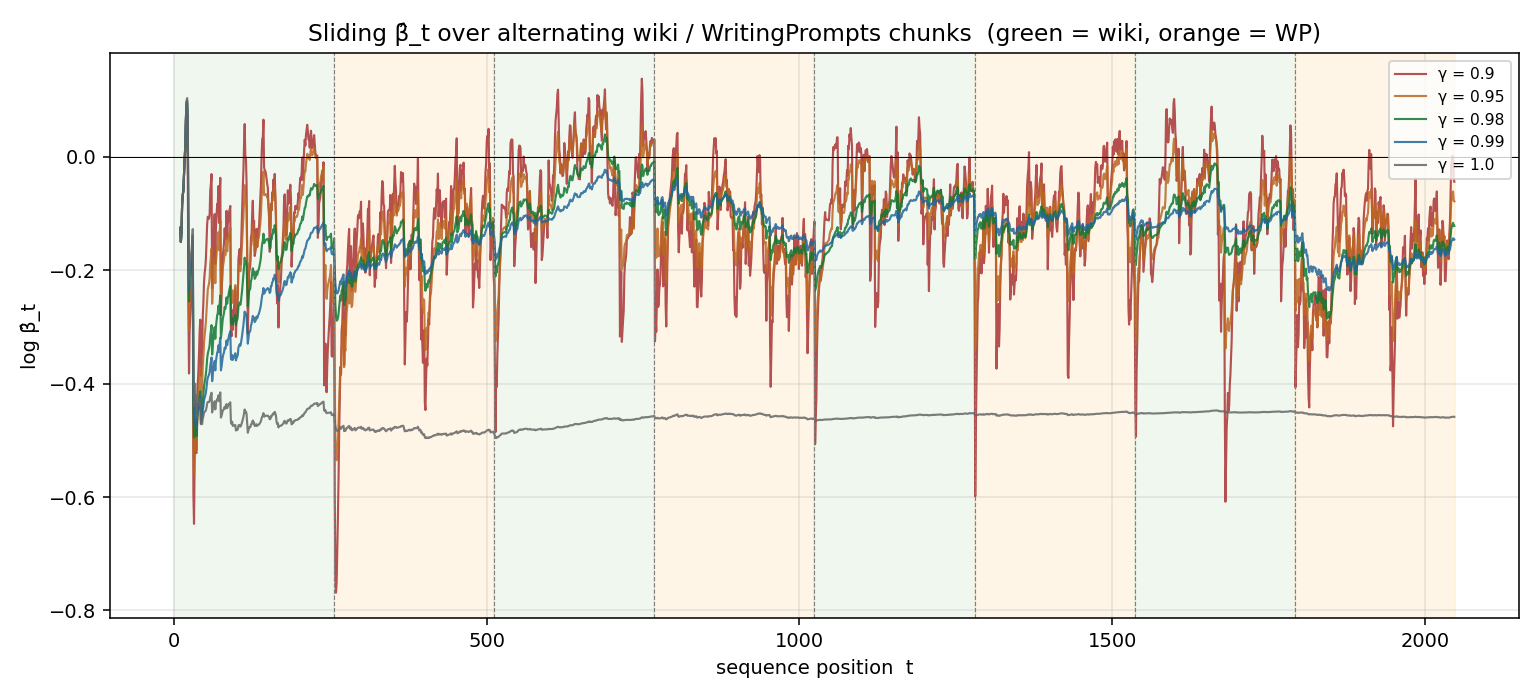
\includegraphics[width=\linewidth]{F_mix_1_log_beta_trajectory.png}
\caption{$\log\hat\beta_t$ as a function of sequence position $t$ for each
$\gamma$.  Background shading is genre: green = WikiText, orange =
WritingPrompts.  $\gamma = 1.00$ (no decay, grey) just drifts to
$\approx -0.45$ and stops tracking content --- the unconditional pooling
bias from Exp A.  Damped filters oscillate.}
\label{fig:mix-traj}
\end{figure}

\begin{table}[h]
\centering
\caption{Mean $\log\hat\beta$ per genre over boundary-stripped chunk
interiors, and mean pre-decoding model entropy $H$ per genre.}
\begin{tabular}{cccccc}
\toprule
$\gamma$ & mean $\log\hat\beta$ wiki & mean $\log\hat\beta$ WP & WT $-$ WP & mean $H$ wiki & mean $H$ WP \\
\midrule
0.90 & $-0.084$ & $-0.138$ & $+0.054$ & 1.686 & 3.024 \\
0.95 & $-0.092$ & $-0.142$ & $+0.051$ & 1.686 & 3.024 \\
0.98 & $-0.115$ & $-0.143$ & $+0.028$ & 1.686 & 3.024 \\
0.99 & $-0.142$ & $-0.140$ & $-0.002$ & 1.686 & 3.024 \\
1.00 & $-0.458$ & $-0.463$ & $+0.005$ & 1.686 & 3.024 \\
\bottomrule
\end{tabular}
\end{table}

\begin{figure}[h]
\centering
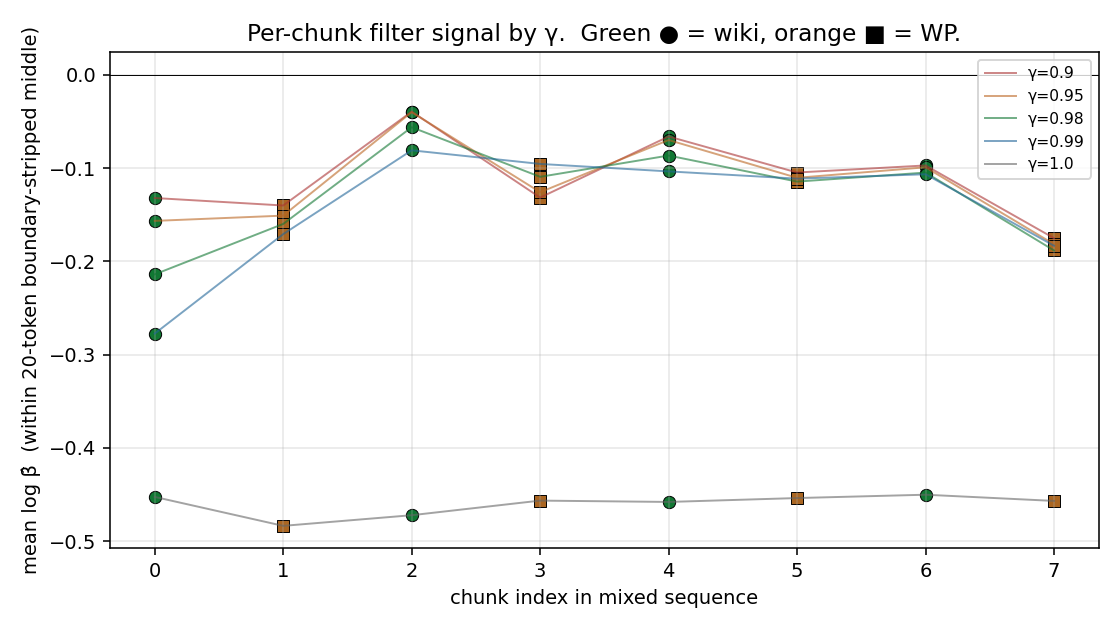
\includegraphics[width=0.85\linewidth]{F_mix_2_gamma_comparison.png}
\caption{Per-chunk mean $\log\hat\beta$ across the 8 chunks in order.
$\gamma = 1.00$ ignores the genre structure entirely (it has saturated to
the unconditional pooled-streaming bias).  Damped filters show some
chunk-to-chunk variation, but the WT--WP gap is small (\, ${\approx}\,0.05$
log units), comparable to within-chunk noise.}
\label{fig:mix-perchunk}
\end{figure}

Three observations.

\paragraph{(a) The damped filter does see a small genre signal.}
At $\gamma = 0.90$--$0.95$, the within-chunk mean of $\log\hat\beta$ is
$\approx 0.05$ log units higher on WikiText than on WritingPrompts.  This
is consistent in sign with the earlier natural\_text/findings result that
the filter's $\hat\beta$ runs slightly negative on WritingPrompts and near
zero on WikiText.  The signal weakens as $\gamma \to 1$.

\paragraph{(b) The genre signal is dwarfed by the entropy signal.}
Pre-decoding model entropy $H$ differs by $\approx 1.3$ nats between the
two genres (1.69 on wiki, 3.02 on WP).  That gap dwarfs the $0.05$-log-unit
filter gap.  Whatever the filter is doing here is mostly tracking some
moderate-bandwidth signal about token predictability, not a sharply
genre-distinct quantity.

\paragraph{(c) $\gamma = 1.00$ saturates to the pooled-streaming bias.}
With no decay, the filter accumulates score and Fisher across the full
2048-token sequence and lands at $\log\hat\beta \approx -0.46$ for every
chunk --- the same one-Newton-step-from-prior-mode artifact established in
Exp A.  Memory decay is necessary if one wants the filter to retain
\emph{any} per-context sensitivity.

\section{Bottom line}

The sliding $\hat\beta_t$ filter at $\gamma = 0.90$--$0.95$ detects a
small ($\approx 0.05$-log-unit) signal that is consistent in sign with
WritingPrompts being apparently lower-$\hat\beta$ than WikiText.  This is
not strong enough to support a per-context calibration claim on top of
Exp A's finding that the filter is not a Guo-style calibrator at all.  At
$\gamma = 1.00$ the filter saturates to its accumulated-bias value and
loses all sensitivity.

What it suggests: the filter's signal here is plausibly content-driven
(higher prefix entropy $\to$ score and Fisher each carry the corresponding
content signature) rather than genuinely about the model's local belief
about its decoder.  Disentangling this from a true decoder-belief signal
would require a controlled experiment varying $\beta_{\mathrm{dec}}$
within a single genre while holding content fixed --- which Exp C
attempted and found dominated by garbage-in/garbage-out off-distribution
drift rather than decoder belief.

\end{document}
